\section{Zielsetzung}
Bei diesem Versuch soll die integrale Energieverteilung sowie das Kontaktpotential des verwendeten
Aufbaus untersucht werden. Außerdem sollen die Anregungsenergie und die Ionisationsenergie von
Quecksilber bestimmt werden.

\section{Theorie}
\subsection{Einleitung}

Der Franck-Hertz Versuch gehört zu den sogenannten Elektronenstoßexperimenten, bei welchen
Atome mit Elektronen beschossen werden und aus den Energiedifferenzen Rückschlüsse auf
die Struktur der Elektronenhülle geschlossen werden.
In diesem Fall werden Elektronen mit möglichst gleichmäßiger Energie in einem abgeschlossenen
Raum auf Hg-Dampf geschossen, wobei zwischen den Elektronen und den Atomen elastische
sowie inelastische stattfinden.
Bei einem inelastischen Stoß werden die Hg-Atome angeregt und nehmen dabei die Energiedifferenz
\begin{equation}
  \frac{\text{m}_0 \text{v}^2_{\text{vor}}}{2} - \frac{\text{m}_0 \text{v}^2_{\text{nach}}}{2} = \text{E}_1 -\text{E}_0
  \label{eqn:Edif}
\end{equation}
zwischen dem Grundzustand mit Energie $\text{E}_0$ und dem ersten angeregten Zustand mit Energie
$\text{E}_1$ vom Elektron auf. Hierbei bezeichnet $\text{m}_0$ die Ruhemasse der Elektronen
und $\text{v}$ die Geschwindigkeit.
Mithilfe der Gegenfeldmethode lässt sich hierbei die Energie der Elektronen messen und
somit diese Energiedifferenz bestimmen.


\subsection{Aufbau}
Der schematische Aufbau des Franck-Hertz-Versuchs ist in Abbildung \ref{fig:Aufbau}
dargestellt.
\begin{figure}[H]
  \centering
  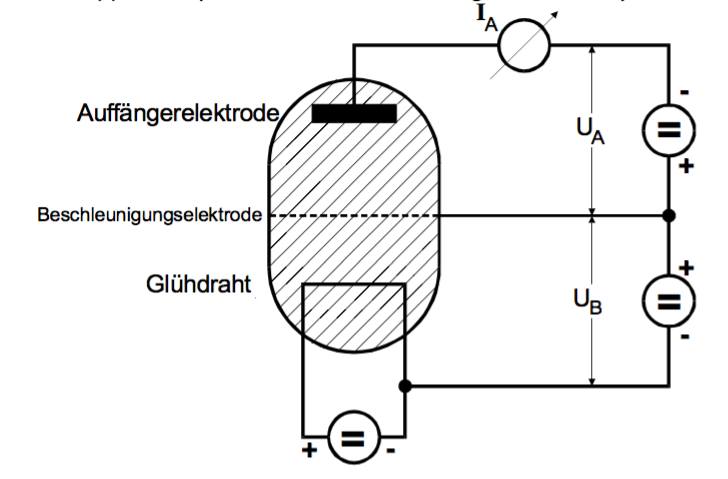
\includegraphics[height=5cm]{Aufbau.png}
  \caption{Aufbau des Franck-Hertz Versuchs \cite{skript}.}
  \label{fig:Aufbau}
\end{figure}
Der Aufbau besteht prinzipiell aus einem evakuierten Gefäß, welches zum Teil mit Quecksilberdampf
gefüllt ist. Es stellt sich hierbei, abhängig von der Umgebungstemperatur, ein Gleichgewichtsdampfdruck
$ \text{p}_{\text{Sät}}$ ein.
In das Gefäß ist zudem ein Glühdraht eigelassen, durch welchen ein Gleichstrom fließt, welcher
mittels des glühelektrischen Effekts dafür sorgt, dass freie Elektronen austreten.
Diese werden dann von einer Beschleunigungsspannung $ \text{U}_B$ zu einer netzförmigen
Elektrode beschleunigt, wobei sie die kinetische Energie
\begin{equation}
  \frac{\text{m}_0 \text{v}^2_{\text{vor}}}{2} = \text{e}_0 \text{U}_B
  \label{eqn:ekin}
\end{equation}
aufnehmen. Hierbei bezeichnet $\text{e}_0$ die Elementarladung.
Hinter dieser Beschleunigungselektrode liegt dann die Auffängerelektrode, an welcher
sich der Auffängerstrom $\text{I}_A$ messen lässt. Wird an dieser nun ein Gegenfeld mit
Gegenspannung $\text{U}_A$ angelegt, können nur noch Elektronen, deren Geschwindigkeitskomponente
in Z-Richtung die Ungleichung
\begin{equation}
  \frac{\text{m}_0 \text{v}^2_{z}}{2} \geq \text{e}_0 \text{U}_A
\end{equation}
erfüllt, gegen die Bremsspannung anlaufen und somit an die Auffängerelektrode gelangen, der Rest
kehrt zur Beschleunigungselektrode zurück. \\
Im Bereich, in dem sich die Hg-Atome aufhalten kommt es nun zu Zusammenstößen mit den Elektronen.
Ist die kinetische Energie der Elektronen gering, kommt es zu elastischen Stößen, bei
denen die Energieabgabe aufgrund des großen Massenunterschiedes vernachlässigbar klein ist,
beim zentralen Stoß beträgt sie beispielsweise nur
\begin{equation*}
  \increment \text{E} = \frac{4\text{m}_0 M}{(\text{m}_0 + \text{M})^2}\text{E} \approx 1,1 \cdot 10^{-5} \text{E} \:,
\end{equation*}
wobei E die Energie des Elektrons angibt.
Wichtig ist hierbei jedoch die Richtungsänderung, die das Elektron erfährt.\\
Beträgt die kinetische Energie des Elektrons aber mindestens die der Energiedifferenz $ \text{E}_1 - \text{E}_0$
zwischen dem Grundzustand und dem ersten angeregten Zustand des Hg-Atoms, kann es auch zu einem
inelastischen Stoß kommen, bei welchem genau der Betrag dieser Energiedifferenz übertragen wird,
und das Hg-Atom wird somit angeregt. Nach einer sehr kurzen Relaxationszeit geht es jedoch, unter
Aussendung eines Lichtquants der Energie
\begin{equation}
  \text{h}\nu = \text{E}_1 - \text{E}_0
  \label{eqn:quant}
\end{equation}
wieder in den Grundzustand über, wobei h das Plancksche Wirkungsquantum und $\nu$ die Frequenz des
Lichts bezeichnet.
Um diesen Effekt zu beobachten, wird $\text{U}_B$ nun langsam erhöht und dabei der Auffängerstrom gemessen.
Sobald $\text{U}_B$ das Gegenpotential $\text{U}_A$ überschreitet, lässt sich ein
starkes Anwachsen des Auffängerstroms beobachten, da immer mehr austretende Elektronen
abgesaugt werden und das Gegenfeld überwinden können. Wird dabei die Elektronenenergie
von $\text{E}_1 - \text{E}_0$ überschritten, kommt es zu inelastischen Stößen, bei denen
die Elektronen einen Großteil ihrer Energie verlieren und somit nicht mehr genügend
Energie besitzen um das Gegenfeld zu überwinden und zur Auffängerelektrode zu gelangen, sodass
der Auffängerstrom abrupt abfällt.
Wird die Beschleunigungsspannung weiter erhöht, können die Elektronen nach dem Stoß allerdings
noch genügend Energie aufnehmen um das Gegenpotential zu überwinden, wodurch der Strom wieder ansteigt.
Dies geschieht so lange, bis das Elektron auch ein zweites mal ein Atom anregen kann, wobei
es erneut fast seine ganze Energie abgibt und der Strom wieder abfällt. Dieser Vorgang lässt sich
noch einige Male wiederholen, wie in Abbildung \ref{fig:kurve} zu sehen ist.
\begin{figure}[H]
  \centering
  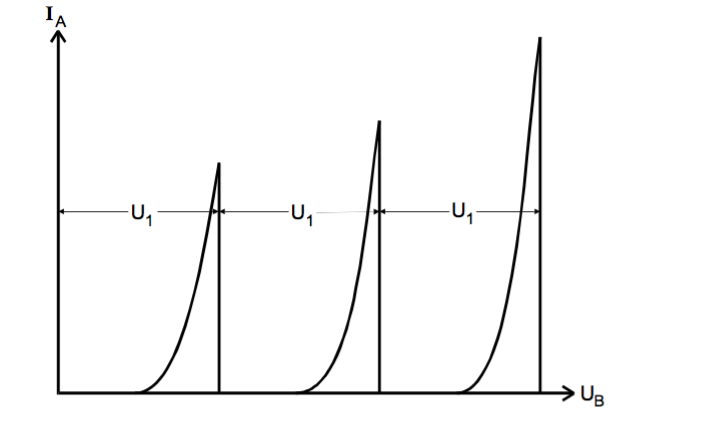
\includegraphics[height=5cm]{Kurve.png}
  \caption{Idealisierte Franck-Hertz Kure \cite{skript}.}
  \label{fig:kurve}
\end{figure}
Der Abstand zweier Maxima beträgt hierbei stets
\begin{equation}
  \text{U}_1 := \frac{1}{\text{e}_0} (\text{E}_1 - \text{E}_0)
\end{equation}

\subsection{Einflüsse auf die Franck-Hertz Kurve}
Eine Idealisierte Franck-Hertz Kurve, wie sie in Abbildung \ref{fig:kurve} dargestellt ist, lässt
sich in der Realität nicht beobachten, was an einer Reihe von Nebeneffekten liegt.
Zum einen weicht die tatsächliche Beschleunigungsspannung $\text{U}_B$ von der von Außen angelegten
Spannung ab, da der Glühdraht und die Beschleunigungselektrode aus verschiedenen Materialien gefertigt
werden und somit jeweils eine unterschiediche Austrittsarbeit besitzen, wodurch ein
Potentialgefälle entsteht, wie in Abbildung \ref{fig:kontakt} dargestellt ist.
\begin{figure}[H]
  \centering
  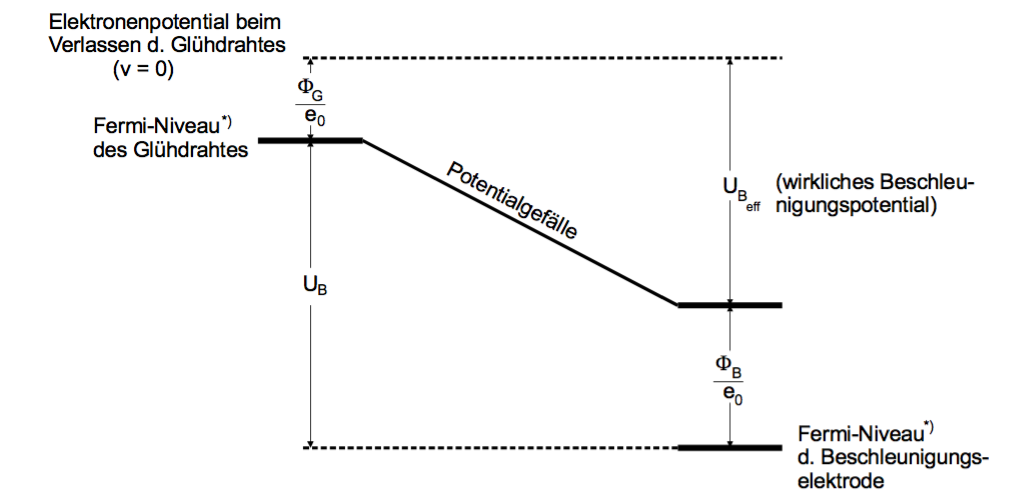
\includegraphics[height=5cm]{Kontakt.png}
  \caption{Potentialgefälle zwischen Glühdraht und Beschleunigungselektrode \cite{skript}.}
  \label{fig:kurve}
\end{figure}
Somit ergibt sich das effektive Beschleunigungspotential zu
\begin{equation}
  \text{U}_{\text{B,eff}} = \text{U}_B - \frac{1}{\text{e}_0}(\phi_B - \phi_G) \: ,
  \label{eqn:ueff}
\end{equation}
wobei der Ausdruck
\begin{equation}
  \text{K} := \frac{1}{\text{e}_0}(\phi_B - \phi_G)
  \label{eqn:kontaktpotential}
\end{equation}
als Kontaktpotential bezeichnet wird und die Verschiebung der Franck-Hertz Kurve
angibt.\\
Zudem haben nicht alle Elektronen, welche aus dem Glühdraht austreten dieselbe
Energie, wie zunächst angenommen, sondern unterliegen der Fermi-Dirac-Verteilung.
Somit besitzen die Elektronen nach durchlaufen der Beschleunigungsspannung nicht eine
feste Energie, sondern ein kontinuierliches Spektrum, weshalb sich nicht genau ein Punkt festlegen
lässt, ab welchem inelastische Stöße stattfinden. Dadurch besitzt die Kurve einen nicht mehr
ganz so starken Anstieg zum Maximum und fällt anschließend auch nicht auf Null, sondern
auf ein Stromminimum ab. \\
Außerdem wird die Kurve auch durch elastische Stöße im Bereich zwischen
Beschleunigungselektrode und Auffängerelektrode abgeflacht und verbreitet, da diese
Art von Stößen Richtungsänderungen verursachen, wodurch es zu einer Verteilung der
Z-Komponente der Geschwindigkeit kommt. Ist die Z-Komponente nun zu klein, erreicht
das Elektron nicht mehr die Auffängerelektrode und wird somit nicht mehr detektiert.\\
Auch der Dampfdruck hat einen Einfluss auf die Gestalt der Franck-Hertz Kurve, denn die
mittlere freie Weglänge $\bar{w}$ sollte etwa um den Faktor 1000-4000 kleiner
sein als der Abstand a zwischen Kathode und Beschleunigungselektrode. Diese ist
über die Gleichung
\begin{equation}
  \bar{w} [\si{\centi\meter}]= \frac{0,0029}{\text{p}_{\text{Sät}}} [\text{p}\text{ in } \si{\milli\bar}]
  \label{eqn:wegl}
\end{equation}
mit dem Sättigungsdruck verknüpft, welcher sich wiederrum durch
\begin{equation}
  \text{p}_{\text{Sät}}(\text{T}) = 5,5 \cdot 10^{7} \exp{(-6876/T)}
  \label{eqn:psat}
\end{equation}
ergibt.
Wählt man die Temperatur so, dass $\text{p}_{\text{Sät}}$ zu klein ist, erreichen
zu viele Elektronen die Auffängerelektrode, die nicht mit einem
Hg-Atom zusammen gestoßen sind. Ist $\text{p}_{\text{Sät}}$ zu groß, finden zu viele
elastische Stöße statt, sodass zu wenig Elektronen das Gegenfeld überwinden können.
